%% Set to false for submission!
\newif\iftodo\todofalse

\documentclass[noacm,acmsmall,anonymous]{acmart}
%\documentclass{article}
\settopmatter{printfolios=false,printccs=false,printacmref=false}
\raggedbottom
\renewcommand\footnotetextcopyrightpermission[1]{} % removes footnote with DOI
\renewcommand{\keywords}[1]{}  % removes "Additional keywords and phrases"
\renewcommand{\acmSubmissionID}[1]{} % removes SUBMISSION ID
\let\oldmaketitle\maketitle
\renewcommand{\maketitle}{
	\oldmaketitle
	\pagestyle{plain}  % empty headers and footers on all pages
	\thispagestyle{plain}  % empty header and footer on the first page
}

\usepackage{array}
\usepackage{graphicx}
\usepackage{multirow}
\usepackage{colortbl}
\usepackage{float}
\usepackage{fancybox}
\usepackage{tcolorbox}
\usepackage{mathtools}
\usepackage{amsmath}
\usepackage{amsthm}
\usepackage{arydshln} % Package for dashed lines
% Disable \Bbbk redefinition if it exists
\let\Bbbk\relax
\usepackage{amssymb}  % for loaner compilation
\usepackage{mathpartir}
\usepackage{geometry}
\usepackage{hyperref}
\usepackage{xcolor}
\usepackage{tikz}
\usepackage{ulem}
\usepackage{cancel} % For middle strikethrough
\usepackage{stmaryrd}
\usepackage{graphicx}    % To include PDF files
\usepackage{subfig}  % To create subfigures
\usepackage{listings}
\usetikzlibrary{petri, positioning}


\newcommand{\jj}[1]{\textcolor{orange}{\textbf{Jules:} #1}}

%\definecolor{ForestGreen}{rgb}{0.13, 0.55, 0.13} % Optional manual definition
%\definecolor{forestgreen}{RGB}{0, 128, 0} produces a darker green.


\definecolor{lightgray}{rgb}{0.9,0.9,0.9}


\geometry{a4paper, margin=1in}

\title{Serializability in Programmable Networking Services}
\author{}
\date{\today}

\definecolor{ForestGreen}{RGB}{34, 139, 34}

% Define the \INITNETWORK command
\newcommand{\INITNETWORK}{\textcolor{ForestGreen}{\textbf{\textsc{INITIALIZE\_NETWORK}}}}
\newcommand{\TERMINATE}{\textcolor{ForestGreen}{\textbf{\textsc{TERMINATE}}}}
\newcommand{\FIRING}{\textcolor{ForestGreen}{\textbf{\textsc{FIRING}}}}
\newcommand{\TOKENPi}{\textcolor{ForestGreen}{\textbf{\textsc{TOKEN}}\_$p_i${}}}
\newcommand{\ADDTOKENPi}{\textcolor{ForestGreen}{\textbf{\textsc{ADD\_TOKEN\_}}$p_i${}}}
\newcommand{\REMOVETOKENPi}{\textcolor{ForestGreen}{\textbf{\textsc{REMOVE\_TOKEN\_}}$p_i{}$}}
\newcommand{\REMAININGINITIALTOKENPi}{\textcolor{ForestGreen}{\textbf{\textsc{REMAINING\_INITIAL\_TOKEN\_}}$p_i${}}}


\newcommand{\SPAWN}{\textcolor{blue}{\texttt{SPAWN}}}
\newcommand{\DONE}{\textcolor{blue}{\texttt{DONE}}}
\newcommand{\DROP}{\textcolor{red}{\texttt{DROP}}}
\newcommand{\observation}{Observation}
\newcommand{\HB}{\sqsubset}
\newcommand{\heapAfterTick}{\mathsf{tick\_clock}}
\newcommand{\sendEvent}{\mathsf{SEND}}
\newcommand{\receiveEvent}{\mathsf{RECEIVE}}
\newcommand{\readEvent}{\mathsf{R}}
\newcommand{\writeEvent}{\mathsf{W}}
\newcommand{\F}{\mathsf{F}}
\newcommand{\Sw}{\mathsf{Sw}}
\newcommand{\yield}{\mathsf{yield}}
\newcommand{\p}{\mathsf{p}}
\newcommand{\s}{\mathsf{s}}
\let\C\relax  % Undefine the existing \C command
\newcommand{\C}{\mathcal{C}}
\newcommand{\T}{\mathcal{T}}
\newcommand{\ifExp}{\texttt{if}}
\newcommand{\elseExp}{\texttt{else}}
\newcommand{\whileExp}{\texttt{while}}
\newcommand{\exit}{\texttt{exit}}
\newcommand{\before}{\mathsf{before}}
\newcommand{\after}{\mathsf{after}}
\newcommand{\packetMatch}{\mathsf{packet\_match}}
\newcommand{\switch}{\mathsf{switch}}
\newcommand{\switches}{\mathsf{switches}}
\newcommand{\spawn}{\mathsf{spawn}}
\newcommand{\send}{\mathsf{send}}
\newcommand{\receive}{\mathsf{receive}}
\newcommand{\receiveAndReconcile}{\mathsf{receive\_and\_reconcile}}
\newcommand{\reconcile}{\mathsf{reconcile}}
\newcommand{\append}{\mathsf{append}}
\newcommand{\Actions}{\mathsf{Actions}}
\newcommand{\LocalState}{\mathsf{LocalState}}
\newcommand{\EventDomain}{\mathsf{Event}}
\newcommand{\event}{\mathsf{event}}
\newcommand{\idx}{\mathsf{idx}}
\newcommand{\cur}{\mathsf{cur}}
\newcommand{\src}{\mathsf{src}}
\newcommand{\Clock}{\mathsf{Clock}}
\newcommand{\VAR}{\mathsf{VAR}}
\newcommand{\var}{\mathsf{var}}
\newcommand{\timeField}{\mathsf{current\_clock}}
\newcommand{\srcField}{\mathsf{src}}
\newcommand{\dstField}{\mathsf{dst}}
\newcommand{\srcClock}{\mathsf{src\_clock}}
\newcommand{\dstClock}{\mathsf{dst\_clock}}
\newcommand{\variableField}{\mathsf{var}}
\newcommand{\valueField}{\mathsf{val}}
\newcommand{\BooleanExp}{\mathsf{Boolean\_Exp}}
\newcommand{\Event}{\mathsf{Event}}
\newcommand{\Exp}{\mathsf{Exp}}
\newcommand{\Thread}{\mathsf{Thread}}
\newcommand{\Heap}{\mathsf{Global\_Heap}}
\newcommand{\State}{\mathsf{State}}
\newcommand{\Pk}{\mathsf{Pk}}
\newcommand{\M}{\mathsf{M}}
\newcommand{\Bag}[1]{\mathsf{Bag}(#1)}
\newcommand{\N}{\mathbb{N}}
\newtheorem{lemma}{Lemma}
% Define corollary environment
\newtheorem{corollary}{Corollary}
%\newtheorem{definition}{Definition}



% Define the lemma and proof environment
%\newtheorem{lemma}{Lemma}[section] % Numbering by section
%\newenvironment{proof}[1][Proof]{\noindent \textbf{#1.} }{\hfill$\square$}

\renewcommand{\paragraph}[1]{\vspace{1mm}\noindent{\bf #1}\ }

\newcommand{\todo}[1]{{\color{red}{\textbf{[TODO]} #1}}}

\newcommand{\nate}[1]{\marginpar{\textcolor{red}{Nate: #1}}}
\newcommand{\jules}[1]{\marginpar{\textcolor{green}{Jules: #1}}}
\newcommand{\guy}[1]{\marginpar{\textcolor{blue}{Guy: #1}}}

\newcommand{\definition}[1]{%
	\vspace{2mm}%
	\noindent%
	\textbf{Definition:} \textit{#1}%
	\vspace{2mm}%
}

%\newtheorem{definition}{Definition}[section] % This creates a definition 
%%environment with numbering by section

%% Disable \Bbbk redefinition if it exists
%\let\Bbbk\relax
%\usepackage{amssymb}    % Load after to avoid conflicts


% Python style for code
\lstdefinestyle{pythonStyle}{
	language=Python,                           % Set language to Python
	backgroundcolor=\color{white},             % Set background color
	basicstyle=\ttfamily\footnotesize,         % Set font to typewriter 
	%(monospace) and size
	keywordstyle=\color{blue}\bfseries,        % Keywords in blue and bold
	commentstyle=\color{purple},               % Comments in purple
	stringstyle=\color{red},                   % Strings in red
	numbers=left,                              % Line numbers on the left
	numberstyle=\tiny\color{gray},             % Line numbers style
	stepnumber=1,                              % Number every line
	numbersep=5pt,                             % Distance between line numbers 
	%and code
	showstringspaces=false,                    % Don't show space characters
	breaklines=true,                           % Wrap long lines of code
	frame=single,                              % Draw a frame around the code
	rulecolor=\color{black},                   % Frame color
	captionpos=b,                              % Set caption position to bottom
	escapeinside={\%*}{*)},                    % Allow LaTeX comments inside 
	%code
	xleftmargin=1em, 
	% Left margin for code 
	%indentation
	% Left margin for code indentation
	keepspaces=true                            % This ensures spaces are kept 
	%in the code block
}

\begin{document}
	


\begin{abstract}
        Add abstract here
\end{abstract}

\maketitle

\section{Introduction}
\label{sec:introduction}

For concurrent systems, from databases to software-defined networks (SDNs), a cornerstone correctness criterion is \emph{serializability}: every concurrent execution must produce outcomes equivalent to some serial ordering of requests. Violations of serializability can lead to subtle anomalies, such as lost updates in databases or routing cycles in SDNs.
While we can check serializability for a fixed number of requests with known execution steps by enumerating all interleavings, the problem is undecidable for general programs, requiring techniques such as runtime verification or incomplete bounded model checking \cite{WaSt06a,WaSt06b,FlFrYi08,FaMa08,SiMaWaGu11a,SiMaWaGu11b,Pa79,AlMcPe96,BiEn19}.

However, \citet{BoEmEnHa13} have shown (as a special case of bounded-barrier linearizability) that the problem is decidable for programs with bounded-size global state and bounded per-request state even for an \emph{unbounded} number of in-flight requests each performing an \emph{unbounded} number of steps. The purpose of this paper is to make this theoretical decidability result a reality by designing practical algorithms that either prove serializability (with a proof certificate) or prove non-serializability (with a counter-example trace).
% 
We illustrate the problem by example:

% examples in Listings~\ref{lst:MotivatingExample1Ser},~\ref{lst:MotivatingExample2NonSer}, and ~\ref{lst:MotivatingExample3Ser}, written in our modeling language called Ser.

\noindent
\begin{minipage}[t]{0.55\textwidth}
	\begin{minipage}[t]{\textwidth}
		\begin{lstlisting}[caption={Without yield or lock (serializable)},
			label={lst:MotivatingExample1Ser}]
  // request handler invoked by clients          
  request main: 
      X := 1 // X is global (uppercase)
      y := X // y is local (lowercase)
      X := 0
      return y 
		\end{lstlisting}
	\end{minipage}
	\vspace{1em}
	\begin{minipage}[t]{\textwidth}
		\begin{lstlisting}[caption={With yield (not serializable)},
			label={lst:MotivatingExample2NonSer}]
  request main: 
      X := 1 
      yield // let another request run
      y := X // can read 0!
      X := 0
      return y 	
		\end{lstlisting}
	\end{minipage}
\end{minipage}%
\hfill
\begin{minipage}[t]{0.35\textwidth}
	\begin{lstlisting}[caption={With yield and lock (serializable)},
		label={lst:MotivatingExample3Ser}]
  request main: 
      // lock
      while (L == 1): 
          yield
      L := 1 

      X := 1
      yield
      y := X 
      X := 0

      // unlock    
      L := 0
      return y 
	\end{lstlisting}
\end{minipage}

These examples are written in our modeling language called Ser.
A Ser program has a set of named \textbf{request handlers} (one handler \texttt{main} in the examples) that are arbitrarily invoked concurrently by the external environment.
Each incoming request processes its request handler's body until it returns a value as its \textbf{response}. Concurrency is managed by the \textbf{yield} statement, which pauses the current request and gives other requests a chance to run. Ser programs have uppercase \textbf{global shared variables} (\texttt{X} in the examples) and lowercase \textbf{request-local variables} (\texttt{y} in the examples).



%
The first program (Listing~\ref{lst:MotivatingExample1Ser}) is clearly serializable because there are no yields, and hence, no interleavings: each \texttt{main} request returns 1.
In the second program (Listing~\ref{lst:MotivatingExample2NonSer}), the yield allows interleavings and is \emph{not} serializable; consider two concurrent requests to \texttt{main}:
\begin{enumerate}
\item Request A executes \texttt{X := 1} then yields to Request B
\item Request B executes \texttt{X := 1}, yields to itself, reads \texttt{X} (getting 1), sets \texttt{X := 0}, and returns 1
\item Request A resumes, reads \texttt{X} (now 0), and returns 0
\end{enumerate}
This produces the multiset \{(\texttt{main}, 0), (\texttt{main}, 1)\} of (request, response) pairs, which is impossible in any serial execution (where all \texttt{main} requests return 1 and never 0).
Of course, having yields does not guarantee that an execution is necessarily not serializable, as observed in the third snippet (Listing~\ref{lst:MotivatingExample3Ser}). This program uses an additional lock variable ``L'', which guarantees that even if an interleaving occurs, the program is semantically equivalent to the first one.
%
These examples demonstrate that reasoning about serializability can be complex even for very simple programs with few requests running concurrently.
\vspace{-.5em}
\paragraph{Problem Definition.}
Formally, we define the \textbf{observable execution} of a Ser program as a multiset of (request, response) pairs. The \textbf{observable behavior} of a Ser program is the set of all possible observable executions that can occur such that the requests are executed concurrently to obtain their paired responses.
A program is \textbf{serializable} if every observable behavior is achievable serially (without interleavings). That is, a Ser program is serializable if its semantics does not change when all yield statements are removed.
%
\emph{The goal of this paper is to design and develop the Ser language and decision procedure for this problem.} In particular, Ser can prove serializability \textbf{automatically} without requiring any manual proof by the user.
\vspace{-.5em}
\paragraph{Challenges.}
To our knowledge, no prior implementation exists that can automatically generate proof certificates for this class of concurrent systems.
Why not?
Our decision procedure builds on Bouajjani et al.'s reduction from serializability to Petri net reachability~\cite{BoEmEnHa13}. However, since Petri net reachability is Ackermann-complete~\cite{CzWo22}, a naive implementation would fail on all but the simplest programs. 
\vspace{-.5em}
\paragraph{Our Approach.}
To address this, we first introduce the abstraction of \textit{network systems} (NS) --- abstract concurrent programs where users send \textit{requests} that manipulate local and shared state before returning \textit{responses}. Ser programs are compiled into NS, on which our decision procedure operates via reduction to Petri net and semilinear set analysis.

As a backend solver, we use SMPT~\cite{AmDa23}, which is a state-of-the-art tool for Petri net reachability.
We note that while our approach is sound (never incorrectly claims serializability), the underlying SMPT Petri Net tool may time out on complex instances, limiting completeness in practice (which is unavoidable for any Petri Net tool, given the Ackermann-completeness of the problem).

We developed several techniques to make the approach practical, including Petri Net pruning, semilinear set compression, and additional manipulations with Presburger formulas.
These optimizations reduce the search space by orders of magnitude, enabling us to successfully verify the serializability of non-trivial programs.

We evaluated our approach on programs with features such as loops, branching, locks, and nondeterminism. Our benchmarks include SDN-inspired examples such as stateful firewalls, BGP routing, and online shopping systems.

To our knowledge, this leads to the first \emph{implemented} decision procedure that: (i) automatically \textit{proves} serializability for unbounded executions; (ii) generates \textit{proof certificates}; and (iii) handles non-trivial programs.


\paragraph{Contributions.}
After a tour of examples in \Cref{sec:tour}, we present the following contributions:
\begin{itemize}
    \item \Cref{sec:problem-definition} introduces the notion of a Network System (NS), a concurrent program abstraction that captures the essence of concurrent systems.
    \item \Cref{sec:formal-results} presents decidability results (a theorem on serializability; two on equivalence), presents the core decision procedure with proof certificates, and presents techniques for semilinear set reductions and Petri-net reductions.
    \item \Cref{sec:implementation} presents the implementation of the Ser toolchain.
    \item \Cref{sec:evaluation} presents case studies on modeling in Ser examples from domains such as SDNs and databases, and presents our extensive evaluation of the toolchain.
\end{itemize}


Finally, we discuss related work in \Cref{sec:related-work} and conclude in \Cref{sec:discussion}.
Our tool, benchmarks, and experiments are available as an anonymous artifact~\cite{ArtifactRepository} and will be permanently hosted with the paper’s final version. There is also a technical appendix accompanying this paper.
\section{Problem Definition}
\label{sec:problemDefinition}

\newcommand{\grammartag}[1]{\qquad\qquad\emph{(#1)}}
\begin{figure}[t]
    \begin{align*}
    \mathbf{Expression}\quad e ::= &&& \\
       | & \quad 0 \mid 1 \mid 2 \mid \ldots                                && \grammartag{Numeric constants} \\
       | & \quad \nondet                                 && \grammartag{Nondeterministic value: 0 or 1}\\
       | & \quad x := e                            && \grammartag{Write to local packet field} \\
       | & \quad x                                 && \grammartag{Read from local packet field} \\
       | & \quad X := e                            && \grammartag{Write to global switch variable} \\
       | & \quad X                                 && \grammartag{Read from global switch variable} \\
       | & \quad e_1 == e_2                        && \grammartag{Equality test} \\
       | & \quad e_1 ; e_2                         && \grammartag{Sequencing} \\
       | & \quad \ifkw(e_1)\{\ e_2\ \}\elsekw\{\ e_3\ \} && \grammartag{Conditional} \\
       | & \quad \whilekw(e_1)\{\ e_2\ \}              && \grammartag{While loop} \\
       | & \quad \yieldkw                      && \grammartag{Yields to scheduler}\\[1em]
    \mathbf{Program}\quad p ::=
        & \quad \requestkw\ name_1\ \{\ e_1\ \}&&\grammartag{Set of request handlers}\\[-0.5em]
        & \quad \qquad \vdots &&\\
        & \quad \requestkw\ name_n\ \{\ e_n\ \}\ 
    \end{align*}
    \caption{Syntax of expressians and programs}
    \label{fig:syntax}
\end{figure}
    
A Network System $\mathcal{N}$ is a tuple $(G, L, \mathit{Req}, \mathit{Res}, g_0, \delta, \mathit{req}, \mathit{resp})$ where:
\begin{itemize}
\item $G$ is a set of global states representing switch state
\item $L$ is a set of local states representing packet contents
\item $\mathit{Req}$ is a set of request events
\item $\mathit{Res}$ is a set of response events
\item $g_0 \in G$ is the initial global state
\item $\mathit{req} \subseteq \mathit{Req} \times L$ is a request transition relation, which describes which requests turn into which packets
\item $\mathit{resp} \subseteq L \times \mathit{Res}$ is a response transition relation, which describes which packets turn into which responses
\item $\delta \subseteq (G \times L) \times (G \times L)$ is a transition relation for packet processing, which describes an atomic step of packet processing that may change the global state.
\end{itemize}

\begin{figure}[t]
    \centering
    \renewcommand{\arraystretch}{1.6}
    \[
    \begin{array}{c}
    \textbf{States and Transitions:}
    \\
    \quad
    \text{A (global) \emph{network state} is a triple }(g,\mathcal{P},M)\text{ where:}
    \\
    \quad
    g \in G \text{ is the current global switch state,}
    \\
    \quad
    \mathcal{P} \in \text{Multiset}(L \times \mathit{Req}) \text{ is a multiset of in-flight packets,}
    \\
    \quad
    M \in \text{Multiset}(\mathit{Req} \times \mathit{Res}) \text{ is a multiset of request--response pairs already completed.}
    \end{array}
    \]

    \[
    \begin{array}{c}
    \textbf{Initial state:}
    \\
    \quad (g_0,\,\varnothing,\,\varnothing)
    \end{array}
    \]

    \[
    \begin{array}{c}
    \textbf{Transition rules:}
    \\[1em]
    \text{(New Request)}\quad\infer{
    (r,\ell)\,\in\,\mathit{req}
    }
    {(g,\;\mathcal{P},\;M) \;\longrightarrow\; (g,\;\mathcal{P} \uplus \{(\ell,r)\},\;M)}
    \\[2em]
    \text{(Packet Step)}\quad\infer{
    ((g,\ell),\,(g',\ell')) \,\in\, \delta
    }
    {(g,\;\mathcal{P} \uplus \{(\ell,r)\},\;M) \;\longrightarrow\; (g',\;\mathcal{P} \uplus \{(\ell',r)\},\;M)}
    \\[2em]
    \text{(Response)}\quad\infer{
    (\ell,s)\,\in\,\mathit{resp}
    }
    {(g,\;\mathcal{P} \uplus \{(\ell,r)\},\;M) \;\longrightarrow\; (g,\;\mathcal{P},\;M \uplus \{(r,s)\})}
    \end{array}
    \]

    \[
    \begin{array}{c}
    \textbf{Complete runs:}
    \\
    \quad (g_0,\,\varnothing,\,\varnothing) \;\longrightarrow\; (g_1,\,\mathcal{P}_1,\,M_1) \;\longrightarrow\; \cdots \;\longrightarrow\; (g_n,\,\mathcal{P}_{n-1},\,M_{n-1}) \;\longrightarrow\; (g_n,\,\varnothing,\,M_n)
    \\[1em]
    \textbf{Interleaved run: } \text{the } \mathcal{P}_i \text{ can have more than one packet, and } \mathcal{P}_n = \varnothing \\
    \textbf{Serial run: } \text{ each } \mathcal{P}_i \text{ has at most one packet, and } \mathcal{P}_n = \varnothing\\
    \text{Int}(\mathcal{N}) = \{ M \in \text{Multiset}(\mathit{Req} \times \mathit{Res}) \mid \exists \text{ interleaved run } (g_0,\,\varnothing,\,\varnothing) \;\longrightarrow^*\; (g_n,\,\varnothing,\,M) \}\\
    \text{Ser}(\mathcal{N}) = \{ M \in \text{Multiset}(\mathit{Req} \times \mathit{Res}) \mid \exists \text{ serial run } (g_0,\,\varnothing,\,\varnothing) \;\longrightarrow^*\; (g_n,\,\varnothing,\,M) \}\\
    \end{array}
    \]

    \caption{State-transition rules for executions of
    \(\mathcal{N} = (G, L, \mathit{Req}, \mathit{Res}, g_0, \delta, \mathit{req}, \mathit{resp})\).
    A transition \(\longrightarrow\) modifies the triple \((g,\mathcal{P},M)\) by either (1) introducing a new request, (2) processing a packet step via \(\delta\), or (3) consuming a packet to produce its response.  When no more steps are possible, the result set \(M\) is the final multiset of request--response pairs that arose during the run.
    Runs are called \emph{serial} if there is at most one packet in flight at any time, whereas \emph{interleaved} runs may have multiple packets in flight at once.}
    \label{fig:network-transitions}
\end{figure}

\begin{definition}[Interleaved executions \(\mathrm{Int}(\mathcal{N})\)]
    Let \(\mathcal{N} = (G, L, \mathit{Req}, \mathit{Res}, g_0, \delta, \mathit{req}, \mathit{resp})\).
    An \emph{interleaved execution} begins in global state \(g = g_0\) with no packets in flight.
    At any point, one may:
    \begin{itemize}
        \item introduce a new request \(r \in \mathit{Req}\), producing an in-flight packet \(\ell \in L\) if \((r,\ell) \in \mathit{req}\);
        \item take an in-flight packet \(\ell\) and transition \(\ell \mapsto \ell'\) and \(g \mapsto g'\) if \(((g,\ell),(g',\ell'))\in\delta\);
        \item consume an in-flight packet \(\ell\) to produce a response \(s\) if \((\ell,s)\in \mathit{resp}\).
    \end{itemize}
    Each request \(r\) must eventually yield exactly one corresponding response \(s\) in a valid execution.
    The set of all finite multisets of \((r,s)\) pairs realizable by such interleavings is:
    \[
        \mathrm{Int}(\mathcal{N})
        \;=\;
        \bigl\{
        M \;\in\; \text{Multiset}(\mathit{Req}\times \mathit{Res})
        \;\mid\;
        M \text{ is realized by some interleaved run of }\mathcal{N}
        \bigr\}.
    \]
\end{definition}

\begin{definition}[Serial executions \(\mathrm{Ser}(\mathcal{N})\)]
In a \emph{serial} execution, requests are processed one at a time:
\begin{enumerate}
    \item Start in \(\,g_0\).
    \item Take a single request \(r\in \mathit{Req}\), convert it to a packet, process that packet until a response \(s\in \mathit{Res}\) is produced.
    \item Update the global state accordingly and repeat with the next request.
\end{enumerate}
No two requests overlap in processing.
The set of all finite multisets of \((r,s)\) pairs realizable by such one-at-a-time runs is:
\[
    \mathrm{Ser}(\mathcal{N})
    \;=\;
    \bigl\{
    M \;\in\; \text{Multiset}(\mathit{Req}\times \mathit{Res})
    \;\mid\;
    M \text{ is realized by some serial run of }\mathcal{N}
    \bigr\}.
\]
\end{definition}

\begin{theorem}[Serializability]
\label{thm:int-eq-ser}
Whether
\(
    \mathrm{Int}(\mathcal{N}) \;=\; \mathrm{Ser}(\mathcal{N})
\)
holds is decidable.
\end{theorem}

\begin{theorem}[Serial Equivalence]
\label{thm:ser-eq-ser}
Whether
\(
    \mathrm{Ser}(\mathcal{N}) \;=\; \mathrm{Ser}(\mathcal{N})
\)
holds is decidable.
\end{theorem}

\begin{theorem}[Interleaved Equivalence]
\label{thm:int-eq-int}
Whether
\(
    \mathrm{Int}(\mathcal{N}) \;=\; \mathrm{Int}(\mathcal{N})
\)
holds is undecidable.
\end{theorem}
Todo
\section{Formulations}
\label{sec:formulations}

The.. 
\section{Proofs}
\label{sec:proofs}

The theorems..


\section{Implementation}
\label{sec:implementation}

We implemented our approach in and en-to-end-tool to be made publicly available with the final version of this paper. Our tool consists in over $20{,}000$ LoC written in \texttt{Rust}.
%
We next elaborate on the architecture of our tool and the various optimizations we added to allow it to run efficiently.

%The implementation..

%\begin{enumerate}
%	\item The extra things we did to make the thing actually run
%	\item Code architecture
%	\item Optimizations
%\end{enumerate}



\subsection{Code Architecture}

\label{subsec:codeArchitecture}

Our tool implements an end-to-end serializability checker for an arbitrary inputs program. If the program is serializable, we return a proof thereof; otherwise, if it is not serializable --- a counterexample is given to the user, for an interleaving that can result to (request,response) pairs that are unattainable in any serial execution.
%
Our workflow translates the decidability problem to an equivalent Petri Net reachability question (for unbounded nets). in which (i) the Petri Net represents all possible interleavings of the problem; and (ii) the reachability query represents a semilinear set (equivalently, a Presburger arithmetic encoding) of all (request,response) pairs that cannot be attained in any serial execution.
%
As Petri Net reachability is Ackermann complete, we added various optimizations to expedite the search process, both in the Petri Net level and the property encoding level.
%
The pipeline of our approach is depicted in Fig.~\ref{fig:full_program_flow}, and includes the following components:
 

\begin{enumerate}
	\item \textbf{Input \& Parsing.} Our model receives one of two textual representation of the program in question: (i) a \texttt{ser} program with the syntax described in Sec.\todo{add}; or (ii) a \texttt{JSON} file which directly encode the transitions of our networking system (NS). Given that the user feeds the former, an additional parsing step takes place, in which the input program is parsed (using the \texttt{parser.rs} module) to an expression tree and then translated to an equivalent networking system. The NS is represented as a struct in the \texttt{ns.rs} module. 
	
	\item \textbf{Petri Net (PN) Conversion.} The NS is the translated into a Petri Net (see the \texttt{petri.rs} module) which represents the interleavings of the NS. Each place represents a local state or a global state, and each token represents a single in-flight request or a terminated response. The PN is encoded in the de-facto standard \texttt{.net} encoding, in order to be compatible with off-the-shelf PN reachability solvers. 
	
	\item \textbf{Semilinear Conversion.} 
	This includes a set of modules (\texttt{kleene.rs}, \texttt{semilinear.rs}, and \texttt{presburger.rs}) which eventually generate a smeilinear set encoding of the non serializable outputs. This conversion is done by the following pipeline: (1) the NS is translated to an NFA encoding all possible (request,response) pairs of the input program; (2) This NFA is translated to a regex (via Kleene's Theorem) and then project (via the Parikh Image) to a semilinear set. The (finite) encoding of the semilinear set symbolically represents all outputs attained via serializable executions of the program, running for an unbounded number of steps; (3) finally, we complement the semilinear set to attain a semilinear set encoding all outputs unattainable via serial executions. At the end of the pipeline, an {XML}-formatted output encodes an LTL reachability query over the PN, which encapsulates constraints over token counts.
	
	
	\item \textbf{Reachability Engine.} The PN and the reachability query are fed to a state-of-the-art PN reachability solver, which runs \textit{Bounded Model Checking} (BMC) in search of a counterexample; and \textit{State Equation} in order to prove reachability. This engine is implemented in the \textit{reachability.rs} and \textit{reachability\_with\_proofs.rs}  modules.
	%
	In order to expedite the reachability search, the we replace the single ``large'' PN and query with multiple smaller PNs, each coupled with a sub-query encoding a separate disjunct in the original query.
	We iteratively solve the disjuncts one-by-one, until reaching \texttt{SAT}, in which case, we have a counterexample; otherwise, if a disjunct is \texttt{UNSAT}, we continue to the next one. If all disjuncts are unsatisfiable, we render the original encoding as unreachable.
	
	
	\item \textbf{Proof \& Certificate Handling.} If the query is \texttt{SAT}, we reconstruct an NS-level non-serializable execution and validates it's correctness. Otherwise, if all disjuncts are \texttt{UNSAT}, our proof module extract an inductive invariant proof for each disjunct. We subsequently ``stich'' these proofs to a single inductive invariant of the full query, and project it to the NS-level, representing a full proof for why serializability holds. Our checker also validates that the inductive invariant is correct, i.e., (i) includes the initial state of the system; (ii) is inductive with regard to the transitions; and (iii) implies that the reachability query is \texttt{UNSAT}, and hence implying serializability. 
	
	
	\item \textbf{Instrumentation \& Logging.} Throughout the pipeline, size and performance metrics (number of places, transitions, constraint complexity, timings) are recorded. The logger outputs structured \texttt{CSV} and \texttt{JSON} logs for later analysis.
	
	\item \textbf{Debug Report Generation.} Finally, a human-readable \texttt{HTML} report is assembled: it embeds the original net, symbolic constraints, reachability results, proof outlines, and profiling graphs. This interactive report allows users to drill down into each transition firing, constraint check, and proof obligation.
	
	\item \textbf{Output Delivery.} The crate exposes a simple CLI and library API. Users obtain either a Boolean reachability verdict (with optional certificate), raw log files, or a full HTML debug report, depending on invocation flags.
	
	\item \textbf{Optimizations.} As we extensively elaborate later, we also include multiple optimizations, both re represent the semilinear sets succinctly, and to prune the PN. These optimizations significantly reduce the search space and expedite the reachability search.
\end{enumerate}



%\noindent
%This linear pipeline - \emph{parse} -> \emph{model} -> \emph{normalize} -> \emph{analyze} -> \emph{prove} -> \emph{report} --- ensures a clear separation of concerns, easy extensibility (e.g., swapping backends), and comprehensive traceability from input to certified result.```


\begin{figure}[htbp]
	\centering
	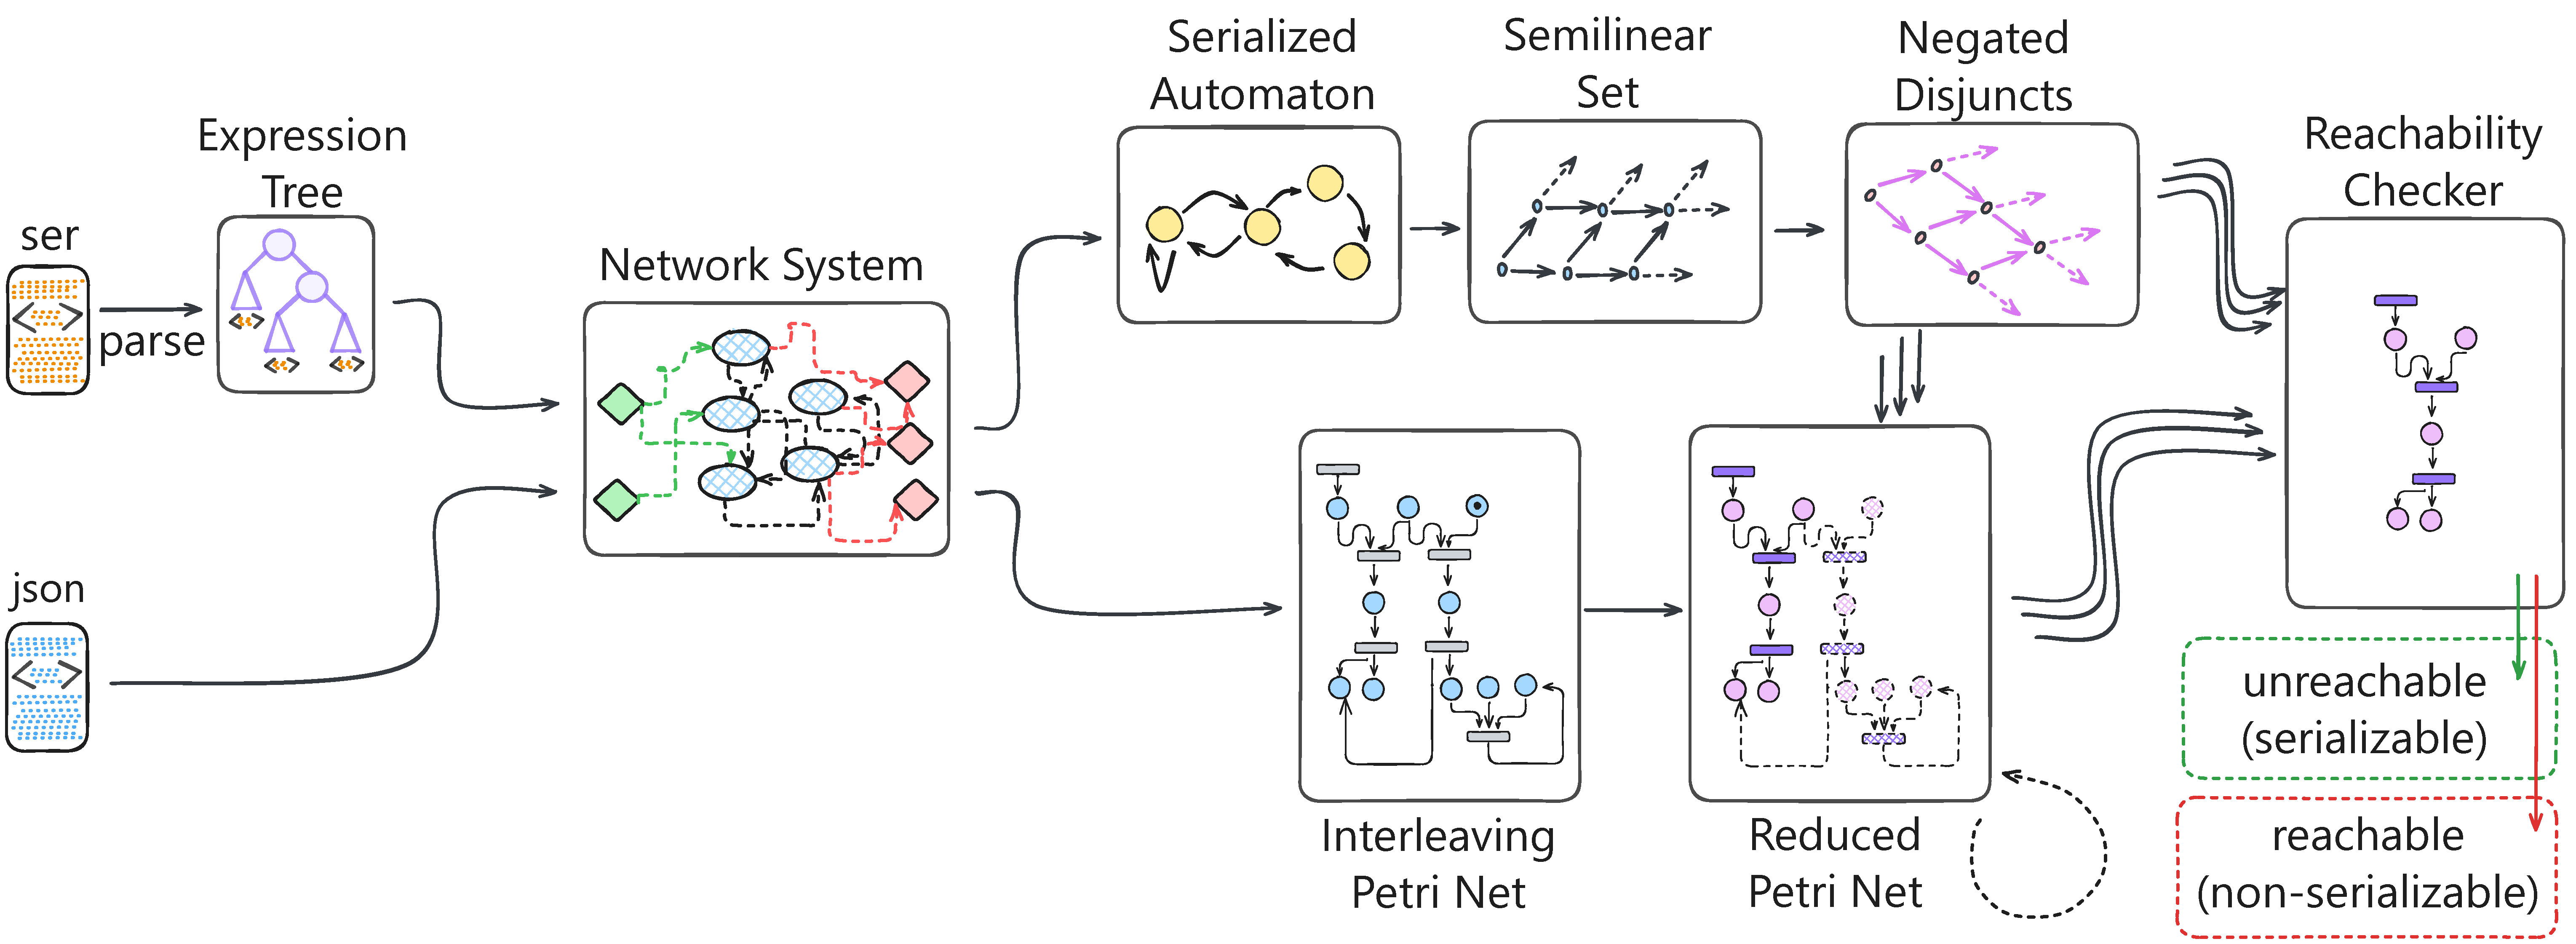
\includegraphics[width=1.0\textwidth]{plots/full_program_flow.pdf}
	\caption{Full program flow. If the program is unreachable --- a serializability proof is produced; otherwise, if it is reachable --- a counterexample trace is generated.
	For simplicity, we omit the backward arrows which translate the invariant found (if serializable) of the counterexample trace (if non serializable) back to the NS level, and to the user.}
	\label{fig:full_program_flow}
\end{figure}


\subsection{Optimizations}

\paragraph{Bidirectional Pruning of the Petri Net}
Before any heavy symbolic reasoning takes place, we apply a bidirectional reachability filter to the underlying Petri net.  In the forward pass, we traverse from the initial marking to identify all places and transitions that could ever fire; in the backward pass, we traverse backward from any place that can influence a target constraint, and identify transitions and places that cannot contribute to reaching it.  By iteratively repeating forward passes and backward passes until convergence, we remove every component of the net that cannot both originate and contribute to the reachable target set.  This dramatically shrinks the net in practice, often converting an intractably large model into one small enough for exhaustive analysis.
%
We give a formal proof of the correctness of this optimization in Appendix~\ref{appendix:BidirectionalProof}.

\paragraph{Redundant‐Constraint Elimination}
When manipulating Presburger sets or their semilinear representations, it is common for some inequalities or disjuncts to add no new coverage beyond what other constraints already guarantee.  The redundant‐constraint elimination pass inspects each linear inequality and each disjunct in a disjunctive normal form, testing whether it is implied by the rest.  Any constraint or disjunct found redundant is dropped, ensuring that subsequent intersection, union, and projection operations work on the smallest necessary formula.  This streamlines the logic formula and prevents exponential blow‐up of case distinctions during solver invocations.
%
%Every time you build or star a semilinear set, you prune out any “period” vectors that are rendered useless by earlier steps:. nce you’ve accumulated a bunch of LinearSet components, you try to merge any that mathematically subsume one another:

\paragraph{Generating Fewer Constraints}
During set‐construction--- especially when introducing new existentially‐quantified variables or combining transition effects, we selectively avoid generating any marking that would strictly dominate an already‐seen solution.  In effect, whenever a candidate disjunct would yield a superset of an existing one, it is skipped entirely.  This ``generate‐less” heuristic stops the proliferation of large, overlapping regions in the semilinear description, trading off completeness of intermediate case‐enumeration for concise final representations.  In benchmarks with large state‐spaces, it can reduce the number of intermediate branches by orders of magnitude.

%in both the Regex and SemilinearSet Kleene-algebra instances. Concretely, instead of always building the full new structure and pruning it later, operations like union (plus) and concatenation (times) do a quick check for trivial cases and drop “zero” or “one” elements on the spo

\paragraph{Executing the Kleene Elimination in a Strategic Order:}
When you converting an NFA to a single regex, we pick the next state to eliminate by heuristically choosing the  state with the fewest incoming and outgoing edges.
This optimization allows circumventing 
overblown expressions resulting in naive translations, especially with regard to  Kleene closures (the “\(\mathsf{*}\)” operator).  Instead, we analyze the structure of subexpressions under the various operators --- estimating their branching factor and likely convergence speed, and reorder them so that simpler, low‐branching components are expanded first.  This adaptive ordering often leads to early detection of fixed points or dead‐ends, preventing the combinatorial explosion that arises when complex loops are expanded prematurely.  




\begin{figure}[htbp]
	\centering
	
	% Top row: (a), (b)
	\begin{subfigure}[b]{0.45\textwidth}
		\centering
		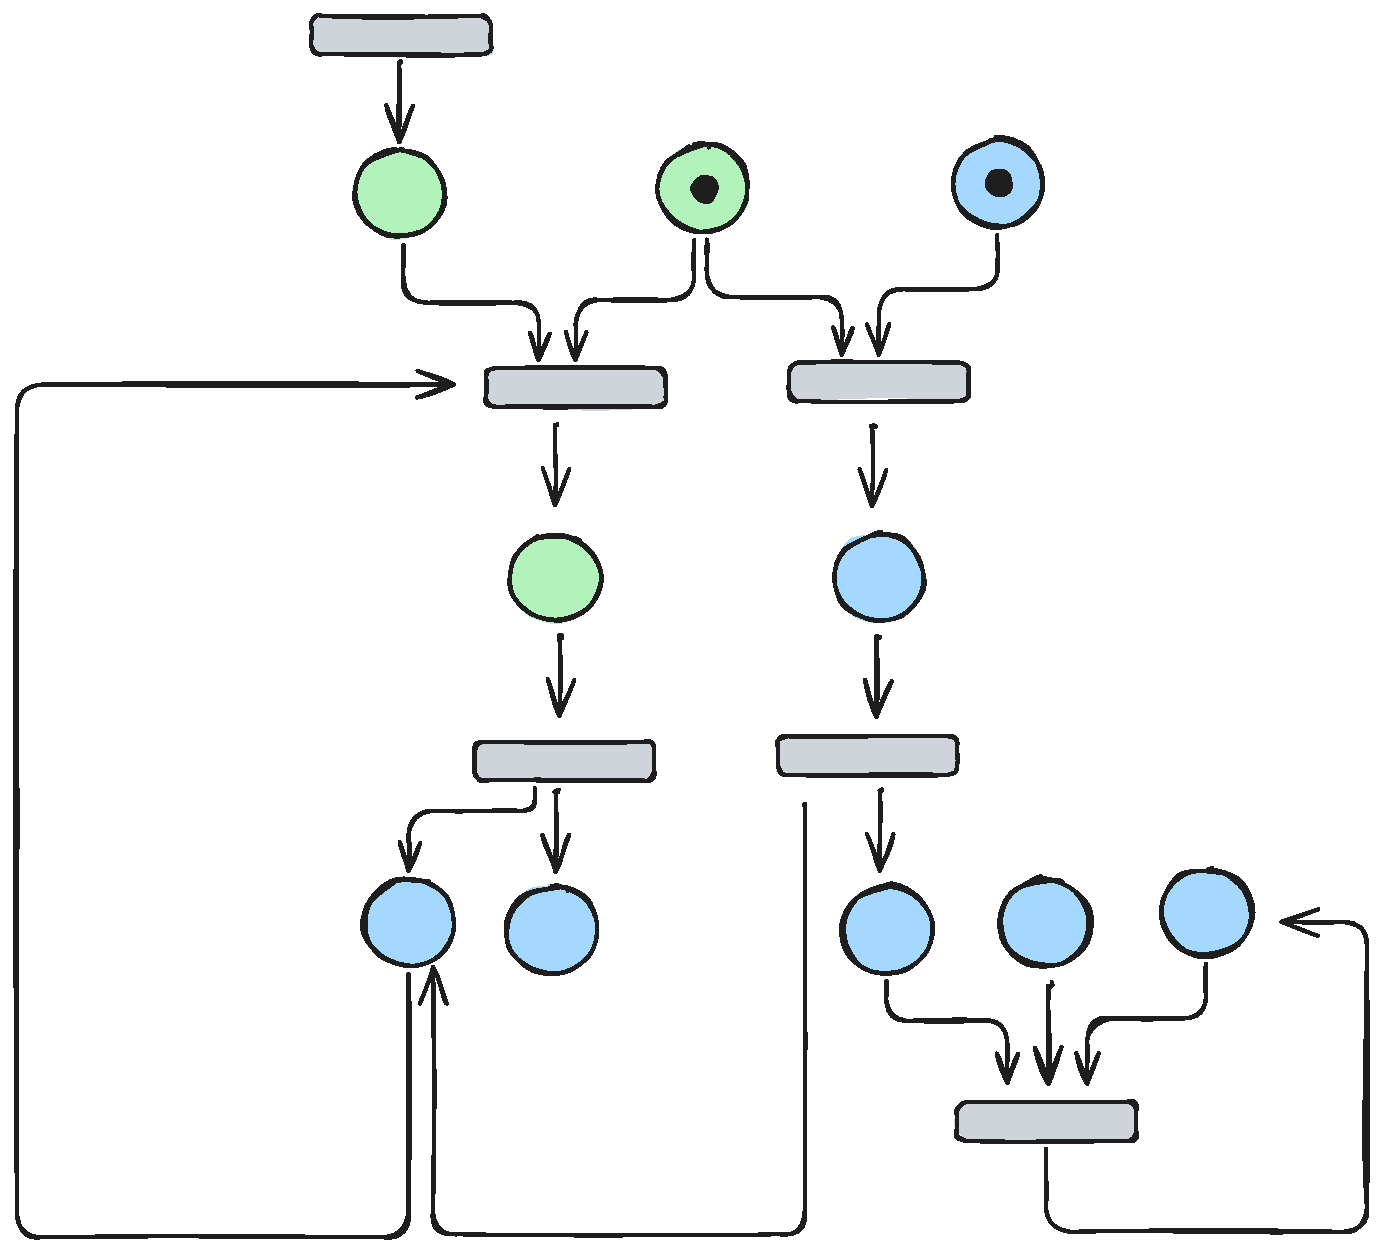
\includegraphics[width=\textwidth]{plots/bidirectional_pruning_step_a_updated.pdf}
		\caption{Step 0: initial petri net, before pruning.}
		\label{fig:step:a}
	\end{subfigure}\hfill
	\begin{subfigure}[b]{0.45\textwidth}
		\centering
		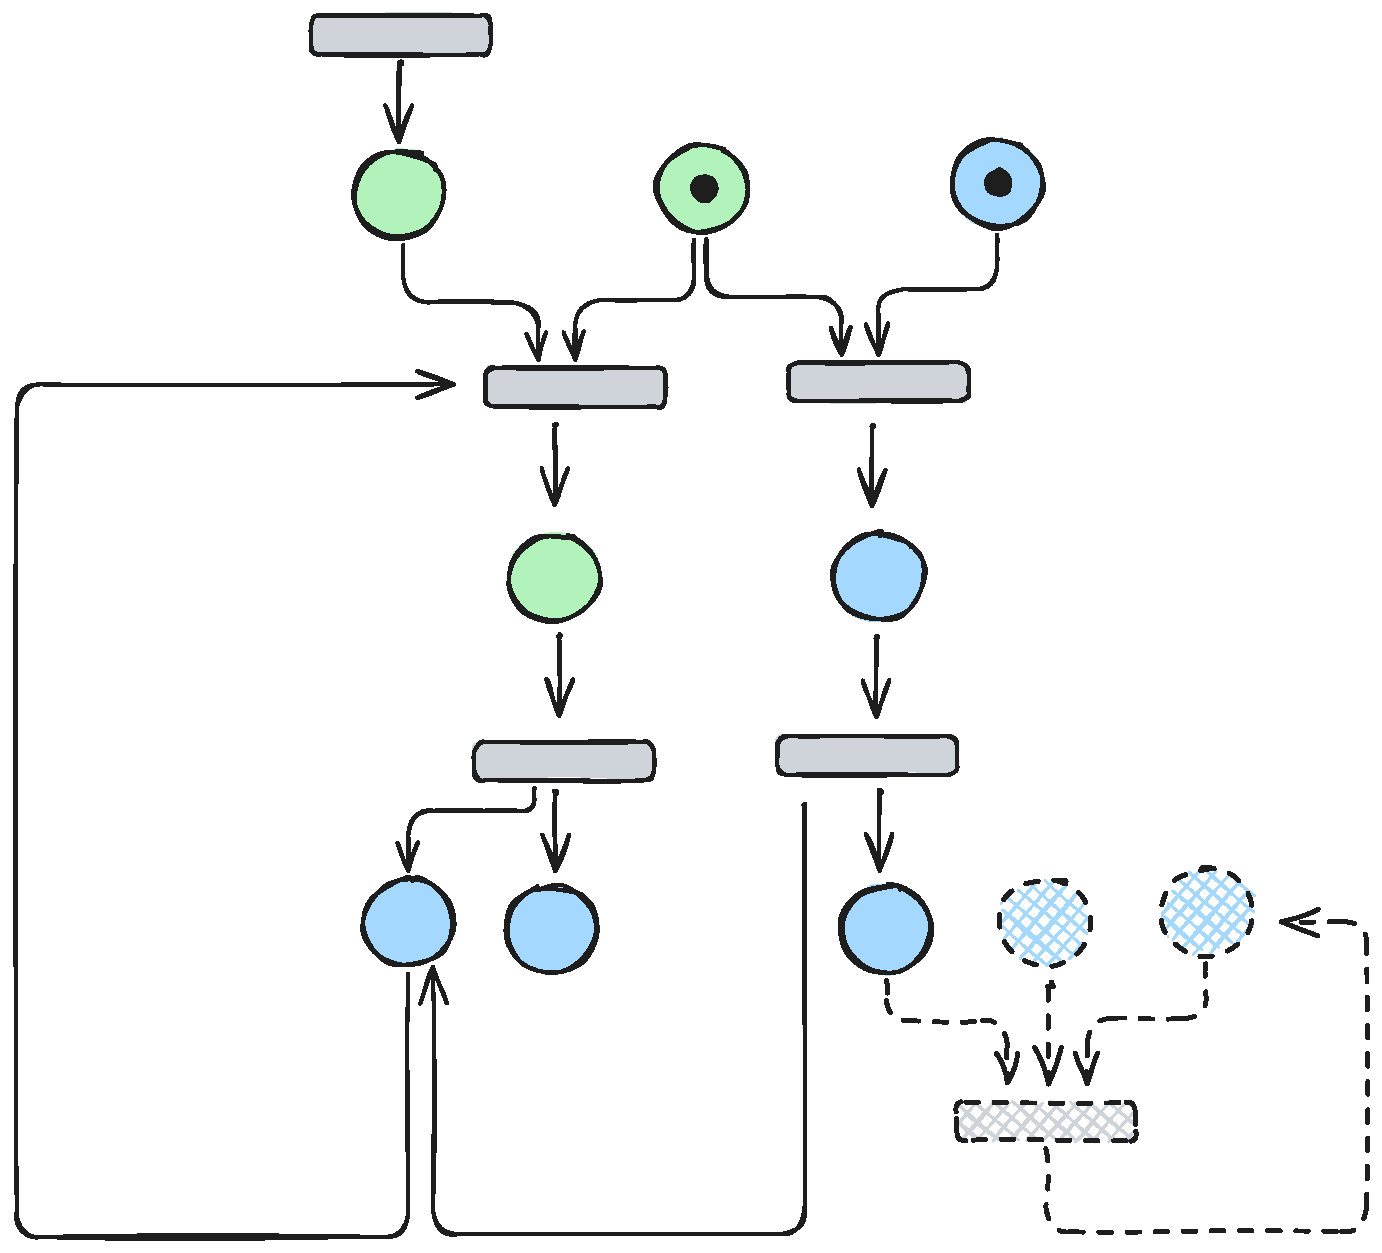
\includegraphics[width=\textwidth]{plots/bidirectional_pruning_step_b_updated.pdf}
		\caption{Step 1: during forward pass.}
		\label{fig:step:b}
	\end{subfigure}
	
	\vspace{1em}
	
	% Bottom row: (c), (d), and (e) matching (d)’s height
	\begin{subfigure}[b]{0.30\textwidth}
		\centering
		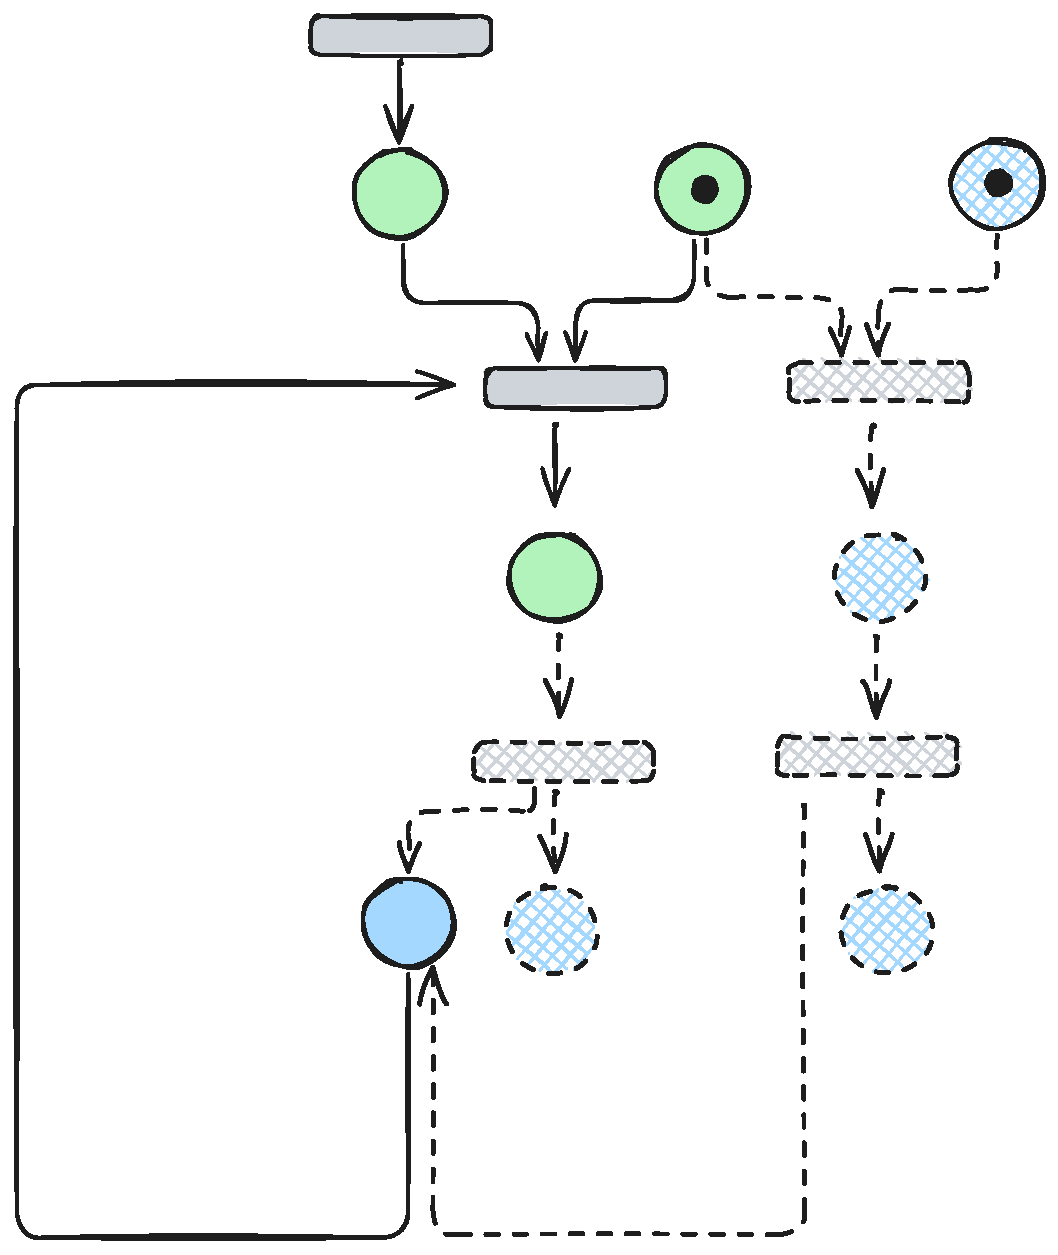
\includegraphics[width=\textwidth]{plots/bidirectional_pruning_step_c_updated.pdf}
		\caption{Step 3: after forward pass, and during backward pass.}
		\label{fig:step:c}
	\end{subfigure}\hfill
	\begin{subfigure}[b]{0.23\textwidth}
		\centering
		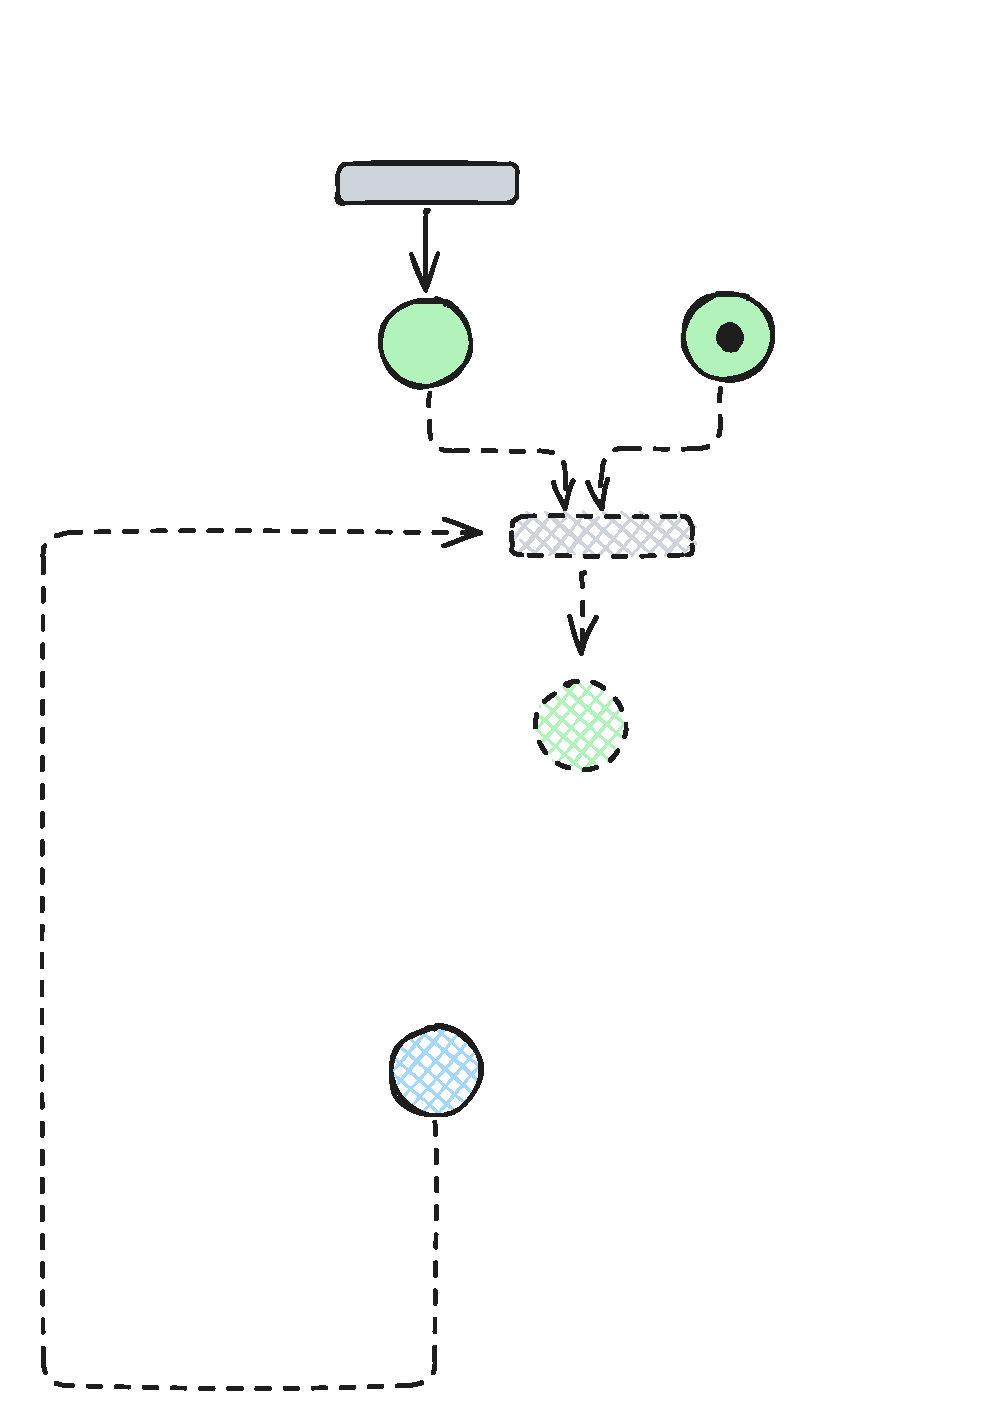
\includegraphics[width=\textwidth]{plots/bidirectional_pruning_step_d_updated_2.pdf}
		\caption{Step 4: after backward pass, and during forward pass.}
		\label{fig:step:d}
	\end{subfigure}\hfill
	% <-- three-arg form: [vpos][total height][inner vpos]
	\begin{subfigure}[b][\subfigheight][b]{0.23\textwidth}
		\centering
		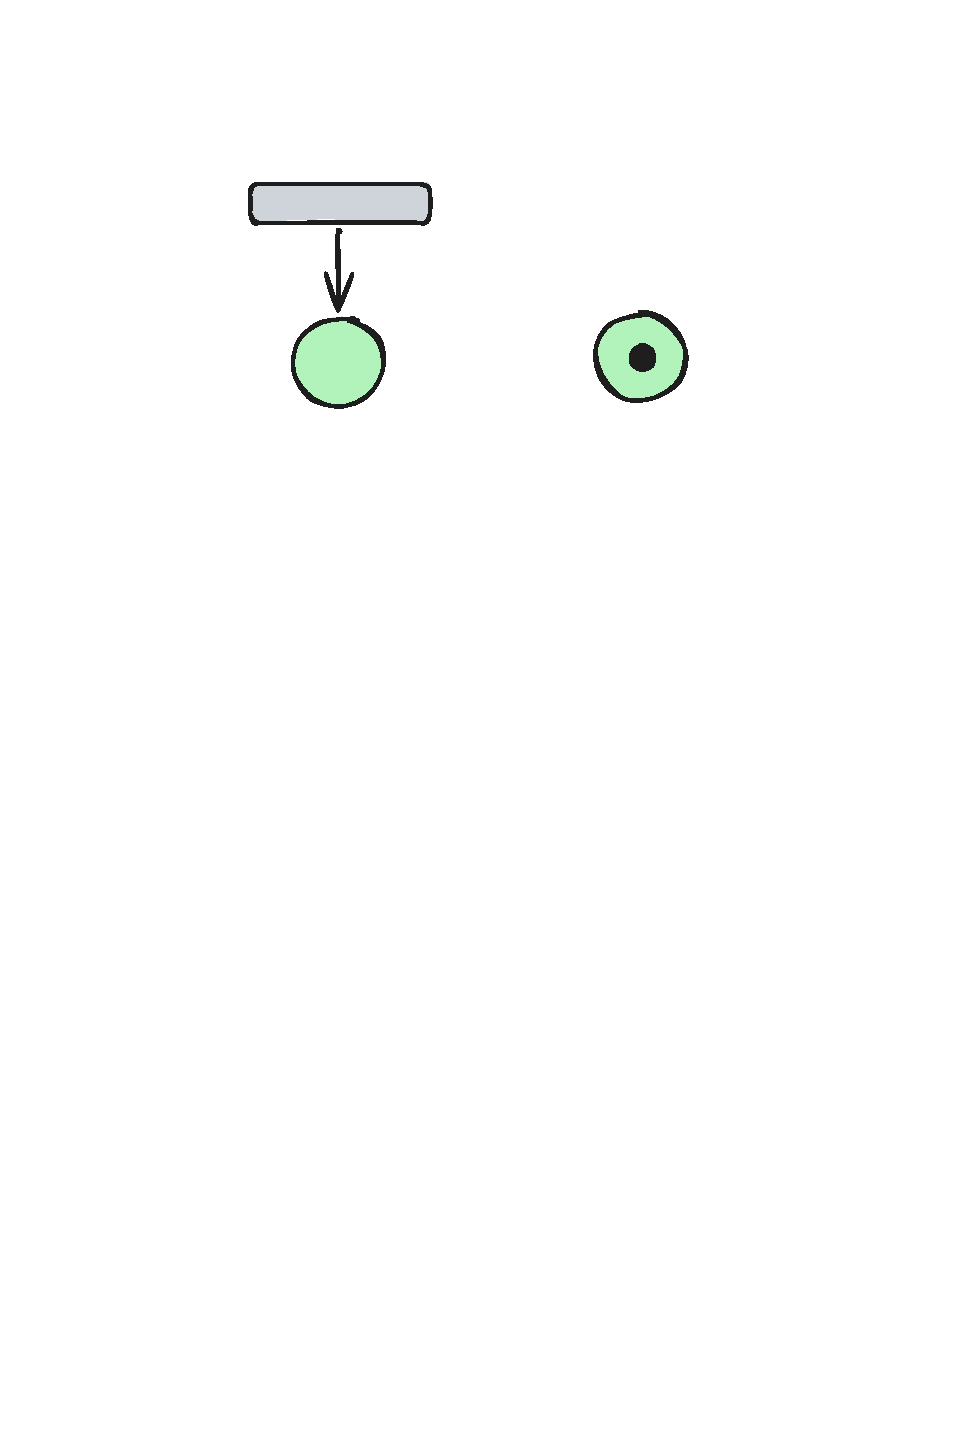
\includegraphics[width=\textwidth]{plots/bidirectional_pruning_step_e_updated_2.pdf}
		\caption{Step 6: final petri net.}
		\label{fig:step:e}
	\end{subfigure}
	
	\caption{A Petri Net after four iterations of bidirectional pruning: two forward passes and two backward passes. Black dots represent initial token markings; green places represent places that are allowed to be reachable in our constraints (i.e., aren't fixed to zero tokens in the final marking). Dashed shapes represent places and transitions that are identified as removable in the current iteration, and will be removed after it ends.}
	\label{fig:bidirectional_pruning}
\end{figure}




%\newpage
\section{Related Work}
\label{sec:relatedWork}

% from the CAV-2010 Vafeiadis paper (+ some other papers in our slack RW thread):
%
%1. model checking techniques - find violations, but do not prove correctness as they work on finite-state systems
%
%2. static (and specifically, shape) analysis techniques (sometimes) work on unbounded threads but ,any of these require linearization points (annotated manually or automatically). Also, a ``failed'' proof can indicate incorrect linearization.
%
%3. manual verification efforts

\subsection{Notions of serializability.}
\label{sec:related:notions-of-serializability}

Serializability (also termed 
\textit{atomicity}) was first formalized by Eswaran et al.~\cite{EsGrKoTr76} as 
a 
correctness condition for concurrent transaction execution. 
Their work also introduced what was later referred to as \textit{conflict 
serializability}, a stricter variant that requires equivalence to a serial 
schedule solely by reordering non-conflicting operations (e.g., two reads by 
different threads). 
%
\textit{Strict serializability} (a.k.a. SSR~\cite{Pa79}) is a stronger 
consistency 
notion in which an execution need not only be serializable but also respects 
the real-time ordering of the transactions, i.e., it is not enough for the 
interleaving to be equivalent to a serial one, but the serial execution must 
also preserve the ordering of the transactions.
%
%Strict serializability:
%
%Guerraoui et al.~\cite{GuHeJoSi08} present a algorithm for model checking 
%strict serializability fro two threads. The work was later 
%extended~\cite{GuHeSi11}, to include a manual proof for an arbitrary number of 
%threads.
%
%Konig and Wehrheim recently proved that it is possible to decide whether 
%all executions of a program are strictly serializable, given that the 
%transactions are live~\cite{KoWe21}.
%
Herlihy and Wing~\cite{HeWe87, HeWi90} defined \textit{Linearizability} as a 
similar notion to that of serializability, but adapted from transactional 
programs 
to concurrent data structures. In this setting, a linearizable data structure 
is one for which every concurrent execution 
with any operations manipulating it, appearing as if the operations occurred 
atomically, while respecting real-time ordering and obeying the object's 
specification. 
%
Equivalently, this can also be viewed as a case of strict serializability in 
which each transaction consists of a single action, operating on a single 
concurrent object~\cite{WaSt06a}.
%
Due to the similarity between serializability and linearizability, we cover 
related work pertaining to both notions.
%
Zhang et al.~\cite{ZhChWa13} relaxed the notion of linearizability to 
\textit{quasi 
linearizability}, and put forth a method to identify violations thereof in 
concurrent data structures.
%
Rastogi et al.~\cite{RaMeBrKoSi93} introduced the notion of 
\textit{predicate-wise serializability} (PWSR), which preserves database 
invariants 
while permitting non-atomic transactions.
%
Other non-serializability-related notions focus on weaker consistency models, 
and include Lamport’s \textit{causal 
consistency}~\cite{La78}, which was later generalized to shared 
memory~\cite{AhNeBuKoHu95} 
and implemented in systems like 
COPS~\cite{LlFrKaAn11}, and inspiring extensive research on model checking and 
complexity analysis~\cite{BoEnGuHa17,ZeBiBoEnEr19,LaBo20}. 


\subsection{Deciding serializability and linearizability}

\subsubsection{Theoretical Results}
%
The \textit{membership problem} of serializability, is deciding whether a 
specific interleaving is serializable. This has been proven to be 
\texttt{NP}-complete 
by Papadimitriou~\cite{Pa79}, a result that was later extended~\cite{BiEn19} to 
other consistency models.
Regarding linearizability, the easier, membership problem is 
\texttt{NP}-complete in 
general, as proven by Gibbons and Korach~\cite{GiKo97}. Their result was later 
extended to \textit{collections}~\cite{EmEn18}.
%\guy{Mark could you check EmEn18?}
%
The \textit{correctness problem} on the other hand, is much harder, and 
pertains to deciding whether \textit{all} executions of a program are 
serializable.
%
While the correctness problem of linearizability is in 
\texttt{EXPSPACE}~\cite{AlMcPe96} when bounding the number of threads, 
 Bouajjani et al.~\cite{BoEmEnHa13} proved that it is undecidable otherwise. 
 The authors also prove that the correctness problem of 
linearizability becomes decidable on the fragment of finite-barrier programs. 
As serializability can be viewed as a case in which there are no barriers, this 
implies that serializability membership is in fact decidable. 
%
In follow-up work, Bouajjani et al. prove that linearizability is decidable 
also 
in the unbounded case for specific abstract state types~\cite{BoEmEnHa18}, in 
which the authors rely on checking coverability in a Vector Addition System 
with States (VASS), which was proven to be in \texttt{EXPSPACE}~\cite{Ra78}.
%
Our work can be viewed as the first tool to implement serializability proofs, 
building upon the theoretical algorithm proposed by Bouajjani et 
al.~\cite{BoEmEnHa13}. While our setting differs from theirs in various aspects 
(e.g., we derive 
the serial specification directly from the program and provide a correctness 
proof; our setting is a transactional distributed system while their setting pertains to a single concurrent object, etc.), the core connection makes our work an implementation of their approach 
in spirit. However, despite the theoretical foundation, the implementation 
itself is the key novelty—translating their algorithm into a practical, 
scalable tool required significant advancements. The process was highly 
non-trivial, demanding various optimizations such as automatic invariant 
inference, automaton minimization, and additional techniques to handle 
unbounded systems efficiently. To the best of our knowledge, ours is the first 
tool capable of verifying serializability in unbounded domains.
%
While these contributions represent significant advances, to our knowledge, our 
work is the first to:
(i) Decide serializability universally --- \textit{considering all executions} 
purely through program semantics and final states, independent of read/write 
conflicts; 
(ii) Support \textit{unbounded} transaction systems; and
(iii) Provide a complete end-to-end implementation.



\subsubsection{Model checking and runtime verification}

In a series of papers, Wang and Stoller put forth runtime techniques for 
detecting violations to serializability~\cite{WaSt06a} as well as fragments of 
serializability such 
as conflict serializability and view-serializability~\cite{WaSt06b}. They do so 
by  checking whether a given execution can be recombined to generate 
non-serializable executions.
%
The expressive Temporal Logic of Actions (TLA)~\cite{La94} is used to encode a 
formal specification that validates whether only serializable executions (or 
conflict-serializable~\cite{CoOlPnTuZu07}) always occur. 
While TLA can naturally encode ``real'' serializability (based on final-state 
equivalence), existing TLA-based approaches~\cite{SoVaVi20, Ho24} remain 
limited to bounded transaction systems. This limitation stems from TLA/TLA+ 
model checkers like \texttt{TLC} and \texttt{Apalache}~\cite{YuMaLa99, 
KoKuTr19}, which require 
finite-state verification and cannot handle unbounded transaction counts.
%
\texttt{Line-up}~\cite{BuDeMuTa10} (built on the \texttt{CHESS} model 
checker~\cite{MuQaBaBaNaNe08}) includes a heuristic-driven technique that 
searches for violations of linearizability by enumerating all possible 
serializations. Similar to spirit is \texttt{LinTSO}~\cite{BuGoMuYa12} which 
search for 
linearizability violations in the Total Store
Order (TSO) weak memory model.
%
\texttt{Violat}~\cite{EmEn19} is a tool that generates tests to identify 
linearizability violations, by 
enumeration linearizations efficiently, per program schema (instead of per 
execution, as in~\cite{BuDeMuTa10}).This follows the authors' previous runtime verification technique~\cite{EmEn18}, which enumerates minimal visibility relations.
%
Additional model checking techniques were proposed by Burnim et 
al.~\cite{BuNeSe11}, which are similar to Line-up~\cite{BuDeMuTa10} but based 
on leveraging bridge predicates~\cite{BuSe09}. 
%
Liu et al.~\cite{LiChLiSuZhDo12} build upon \texttt{PAT}~\cite{SuLuDoPa09} 
(also used 
in~\cite{LiChLiSu09, Zh11}) and verify linearizability through the lens of 
refinement checking optimization, for a finite number of threads.
%
%\guy{Mark, could you please check LiChLiSu09,Zh11}
%
Recently, Golovin et al.~\cite{GoKoVa25} presented \texttt{RELINCHE}, a model 
checker for bounded-linearizability, in which a predefined number of operations 
can be invoked invoked.
%
Other automatic linearizability checking tools include the \texttt{CDSSpec} 
specification checker under the C/C++ 11 memory model, and 
\texttt{Lincheck}~\cite{KoDeSoTsAl23} for verifying linearizability in JVM by 
Ou and 
Demsky~\cite{OuDe17}. 
%
Burckhardt et al.~\cite{BuAlMa07} employ a SAT solver and check for 
linearizability violations of specific client programs.
%
We also note the symbolic-reasoning-based (incomplete) approach by Emmi et 
al.~\cite{EmEnHa15} to identify violations of \textit{observational refinement} 
--- a property equivalent to linearizability in some settings~\cite{FiOhRiYa10, 
	BoEmCoHa15}.
%
As far as we are aware, unlike our algorithm, none of these tools afford 
complete coverage for the case of unbounded threads.
%
Other model checking techniques (e.g.,~\cite{Fl04}) rely on specifying 
\textit{linearization points} (a.k.a. commit points), i.e., points in which the 
event occurs logically. We note 
that identifying all such points can be quite challenging~\cite{VeYaYo09}.
%
These include the work of Vechev et al.~\cite{VeYaYo09}, built upon 
\texttt{SPIN}~\cite{Ho97}, and extending the authors' \texttt{PARGLIDER} 
tool~\cite{VeYa08}.~\footnote{Note that Vechev et al. can also apply their 
technique without linearization points, but solely on bounded executions.}



\subsubsection{Stataic analysis}

Static analysis techniques may prove linearizability for the 
bounded~\cite{AmRiReSaYa07, BeLeMaRaSa08, MaLeSaRaBe08} and unbounded 
cases~\cite{BeLeMaRaSa08, Va09, 
	Va10}, but typically rely on heuristics and the manual/automatic annotation 
	of 
linearization points. 
%
Lian and Feng~\cite{LiFe13} propose a sound program logic that can prove 
linearizability with non-fixed linearization points.
%
Other techniques that depend on linearization points 
include~\cite{OhRiVeYaYo10, ZhPeHa15, AbJoTr16}. 
%
%\guy{Mark can you take a look at Va10, LiFe13, and ZhPeHa15?}
%
We note that both the model-checking techniques (e.g.,~\cite{CeRaZuChAl10}) and 
the static analysis techniques which rely on linearization points are 
inconclusive, as any failed proof can be due to incorrect annotation of the 
linearization points, as previously observed~\cite{BoEmCoHa15}.
%


\subsubsection{Manual proofs and results for specific data types}

Tasiran~\cite{Ta08} proved serializability of the \texttt{Bartok STM}, and 
Colvin et 
al.~\cite{CoGrLuMo06} prove that a list-based set algorithm is linearizable by 
simulating the observed behavior with input/output automata.
%
%\guy{Mark could you take a 2nd look at CoGrLuMo06? Not sure if this is 
%considered manual. One paper which I put in the slack channel mentioned that it 
%semiautomatically verifies linearizability of an implementation.}
%
Other methods demonstrate that in some cases, proofs can be simplified for specific data structure to which certain properties hold~\cite{BoEmEnMu17, FeEnMoRiSh18}.
%
Additional verification attempts of linearizability have been presented both 
with (e.g.~\cite{CoGrLuMo06}) and without (e.g.~\cite{DoGrLuMo04}) the use of 
proof assistants.
%
Linearizability has also been proven for specific data types. For example. 
Wing and Gong~\cite{WiGo93} prove it for  (unbounded) FIFO queues, (unbounded) 
priority queues and other data structures. Chakraborty et al.~\cite{ChHeSeVa15} 
later provided a method for checking linearizability of queue-based algorithms, 
without the use of linearization points. Cern{\`y} et al.~\cite{CeRaZuChAl10} 
present \texttt{CoLT}, a model checker for linearizability of singly-linked 
heap-based 
objects. However, their approach is complete only with regard to a bounded 
number of threads. 
%
Bouajjani et al.~\cite{BoEnWa17} present a recursive algorithm for identifying 
linearizability violations in priority queues (based on register automata), in 
a method similar to the one for finding linearizability violations in stacks 
and (regular) queues~\cite{BoEmEnHa18}.
%


\subsubsection{Additional approaches}

%
Some methods combine multiple approaches, e.g., Shacham et 
al.~\cite{ShBrAiSaVeYa11} use dynamic analysis to identify 
violations of linearizability in concurrent data structures, and combine it 
with a manual proof when their technique did not find a violation.
%
Other techniques attempt to generate tests for linearizability~\cite{WiGo93, 
PrGr12, PrGr13, EmEn17}. For example, 
Lowe~\cite{Lo17} presents a testing framework for linearizability by randomly 
generating histories and subsequently testing if they are 
linearizable.
%
There has also been ample research in technique for linearizability  and simplifying proofs for data structures pertaining ~\cite{BoEmEnMu17, FeEnMoRiSh18, EnKo24} 
%
Other techniques for linearizability proof include the use of theorem provers, 
e.g.~\cite{CoDoGr05, DeScWe11} and proof assistance techniques~\cite{EnKo24}.
%
%\guy{Mark EnKo24 is the OOPSLA paper, is it legit to cite it as a proof assistance technique?} 
%Additional related work includes~\cite{BoEmEnMu17, FeEnMoRiSh18, EnKo24}.
%
%EnKo24: OOPSLA paper (Mark) trying to formalize and prove existing reduction techniques, and introduce a new abstraction for splitting linearizability checking scenarios (cases) and check if they covers all the checks. They don't actually check linearizability but say there it can help other checkers

%FeEnMoRiSh18 simplify proofs for some types of data structures

%BoEmEnMu17 also show that proof can be simplified sometimes 


\section{Deciding conflict serializability}

\subsubsection{Runtime enforcement}
Although conflict serializability is a more conservative measure than 
serializability, it is easier for database schedulers to enforce during 
runtime, either by \textit{pessimistic} locking approaches~\cite{BeHaGo87}, or 
\textit{optimistic} locking 
approaches~\cite{KuRo81, BuMo06}.
%
Both approaches ensure acyclicity in the conflict graph --- a necessary and 
sufficient condition for conflict serializability~\cite{SiMa10}. However, 
because these approaches \textit{ignore program semantics}, these may 
incorrectly reject executions that, although not conflict-serializable, are 
still valid serializable executions, i.e., have the same result as a serial 
execution. 
%
We note that the subject matter of this work is around the notion of (``real'') 
serializability, which takes 
into account the program semantics, and regards whether the final result of the 
program can be attained by a serial execution.
%

\subsubsection{Theoretical results}
From the theoretical perspective, Alur et al.~\cite{AlMcPe96} established that 
correctness problem for conflict serializability is decidable (and in 
\texttt{PSPACE}) 
for bounded transaction systems. Bouajjani et al.~\cite{BoEmEnHa13} later 
proved that decidability also holds in the unbounded case (and 
\texttt{EXPTIME}-complete). Their key insight reveals that while the conflict 
graph 
becomes infinite, cycle detection, and thus conflict serializability, is 
independent of the transaction count. 
%
%By modeling transactions via Vector Addition Systems (equivalent to Petri 
%Nets), they provide a finite framework for analyzing infinite behaviors. This 
%approach inspired our use of Petri Nets to capture Int(S).
%
\subsubsection{Approaches and techniques}

Various works focus on checking conflict serializability, e.g., Farzan and 
Mahusudan~\cite{FaMa08} present a monitoring-based decision procedure for 
conflict serializability of a bounded number of operations, and Flanagan et 
al.~\cite{FlFrYi08} present \texttt{Velodrome} --- a dynamic analyzer for 
conflict 
serializability. Additional dynamic approaches include~\cite{FlFr04, XuBoRa05, 
WaSt06a, CoOlPnTuZu07, EmMaMa10, SiMaWaGu11a} and others.
%
%Other works~\cite{XuBoRa05} have also put forth techniques to automatically 
%detect conflict-serializability violations.
%
Hatcliff et al.~\cite{HaRoDw04} demonstrate the use of the \texttt{Bogor} model 
checker~\cite{RoDwHa03} and check atomicity w.r.t. Liptopn's reduction theory 
of left/right movers~\cite{Li75} (which is reminiscent of 
conflict-serializability).
%
Elmas et al.~\cite{ElQaSeSuTa10} also use the notion of movers and present an 
(incomplete) technique to prove linearizability by iteratively rewriting an 
input program.
%
%\guy{Mark can you please check out ElQaSeSuTa10}
%
Nagar and Jagannathan~\cite{KaJa18} presented an 
automatic static analysis technique to find violations of conflict 
serializability.
%
Sinha et al.~\cite{SiMaWaGu11b} present a sound and incomplete predictive 
analysis technique for detecting violations of conflict serializability, 
following the previous work of Sinha and Malik~\cite{SiMa10} which put forth a 
runtime conflict serializability checker.
%
Von Praun and Gross~\cite{VoGr04} present an unsound static analysis technique 
for identifying potential atomicity violations. Additional static analysis 
techniques are based on type systems, e.g.~\cite{FlQa03, FlFrLiQa08}.
%
Brutschy et al.~\cite{BrDiMuVe17} present a dynamic analysis algorithm and a 
tool that checks whether a given program execution is conflict serializable, in 
an eventually consistent data store. In a follow-up work~\cite{BrDiMuVe18} 
further bridges these concepts by statically detecting 
non-(conflict)-serializable behaviors in causally consistent databases.
%
%Rinetzky et al.~\cite{RiBoRaSaYa} present a conservative static analysis 
%techniques for verifying view-serializability on specific program sub-types.
%
%\guy{Mark, please see my masked comment on RiBoRaSaYa. Do we need to mention 
%	them?}
%
We also note that conflict serializability has been studied in relation to weak 
memory models~\cite{EnFa16}.
%





\subsection{Petri Nets, VAS(S), Semilinear sets  \& Presburger arithmetic.}
\label{sec:related:petri}

In addition, our work builds on both theoretical and practical advances in 
Petri Net research~\cite{Mu89, Es96, Re12, EsNi24}. 
%The undecidability we prove 
%for equivalence of interleavings stems from Hack’s seminal result~\cite{Ha76, 
%HaThesis76} showing the undecidability of reachability set equivalence for 
%Petri Nets. This undecidability originates in a series of reductions from 
%Hilbert’s 10th problem, specifically the possibility of determining whether 
%there exists an integer root for Diophantine equations, a problem that was 
%later proven undecidable by Matijasēvič~\cite{Ma70}.
%%
%Jančar~\cite{Ja95} later provided an alternative proof to this undecidability 
%result, by showing that Petri Nets can simulate universal (and thus 
%undecidable) 2-counter Minsky machines~\cite{Mi67}. In addition, Jančar further 
%strengthened the original result by proving that undecidability holds even for 
%Petri nets with just five unbounded places.
%
%Furthermore, our approach also builds on 
as well as Petri Net reachability algorithms, 
which determine whether a given marking is attainable. While the solution is 
straightforward for bounded nets (through exhaustive enumeration), the solution 
for the unbounded case is highly nontrivial, and was first solved by 
Mayr~\cite{Ma81}, with subsequent improvements by Kosaraju~\cite{Ko82} and 
Lambert~\cite{La92}. Recent work~\cite{CzWo22} has also established this 
problem is \texttt{Ackermann}-complete, implying that, although decidable, it 
is practically infeasible to solve on large nets in the worst case.
%
These theoretical advances in Petri Net reachability have given rise to a 
plethora of practical tools, including \texttt{KReach}~\cite{DiLa20}, 
\texttt{DICER}~\cite{XiZhLi21}, \texttt{MARCIE}~\cite{HeRoSc13}, and others. 
%
Specifically, our implementation leverages \texttt{SMPT}~\cite{AmDa23}, a 
state-of-the-art Petri Net reachability tool that combines SMT-solving with 
structural invariants~\cite{AmBeDa21, AmDaHu22}. At a high level, SMPT 
formulates reachability as satisfiability queries (dispatched to the 
\texttt{Z3} 
solver~\cite{DeBj08}) while curtailing the search space~\footnote{As far as we 
aware, the only two sound reachability solvers for unbounded Petri Nets are 
\texttt{KReach}~\cite{DiLa20} and \texttt{SMPT}~\cite{AmDa23}. Although only 
\texttt{KReach} is claimed as possibly complete, we decided in our 
implementation to use \texttt{SMPT} as it was 
reported~\cite{Am23} that \texttt{KReach} is unable to solve various 
reachability 
problems. 
Still, our Petri Nets are encoded in the standard \texttt{.nnet} format, and 
the property file is encoded in the standard \texttt{.XML} format --- in order 
for our tool to be compatible with any off-the-shelf solvers.
}.
%
%We refer the reader to a survey by Esparza and Nielsen~\cite{EsNi94} (recently republished in~\cite{EsNi24}) for a comprehensive summary of additional decidability results pertaining to Petri Nets.
%
Finally, we believe that our various, nontrivial optimizations, and first and 
foremost --- the automatic invariant inference, are interesting in their own, 
allowing the speedy termination of queries that otherwise timed-out. 

 
 






%Serializability first introduced by Eswaran et al.~\cite{EsGrKoTr76}. It is the first to put forth serializability as a correctness condition for concurrent transaction execution.
%The paper also covers conflict serializability --- a strictly stronger consistency property than serializability, that does not only require that the final state of the system be attained by an equivalent serial execution, but also, that this equivalence be attained by allowing only specific (``non-conflicting'') operations to be reordered.
%%
%Papadimitriou~\cite{Pa79} proved that it is NP-hard to decide whether even the history of a single interleaving is serializable. 
%%
%Moreover, although conflict serializability is more conservative measure than serializability, it is easier to enforce during runtime by various approaches. 
%%
%These approaches are typically categorized as either \textit{pessimistic} locking approaches, e.g, 2-Phase Locking~\cite{BeHaGo87}, or alternatively --- \textit{optimistic} locking approaches, e.g., Optimistic Concurrency Control (OCC)~\cite{KuRo81, BuMo06}.
%%
%
%Furthermore, most work, both in theory and in practice, focuses on proving theorems on conflict serializability, due to is being more straightforward, and corresponding to the programs dependency graph, and \textit{without taking the actual semantics into account}.
%%
%Alur et al.~\cite{AlMcPe96} cover the complexity for deciding conflict serializability, given a bound on the number of transactions. 
%%
%This work was later continued by Bouajjaniet al.~\cite{BoEmEnHa13}, which demonstrate that the problem of deciding whether a program with an \textit{unbounded} number of transaction is conflict serializable, is also decidable and is EXPTIME-complete. The authors show that although the conflict graph in such a case is infinite (and hence, infeasible to traverse) --- conflict serializability can still be decided as the size of the cycle (if it exists), surprisingly, does not depend on the number of transactions. The authors also emulate multiple transactions in a shared memory system with a Vector addition system, and equivalent object to a Petri Net. We took inspiration by defining a Petri Net to capture Int(S). 
%
%In another line of work, there is an attempt to \textit{directly} validate (regular, non-conflicting) serializability by encoding this specification in the highly expressive \textit{Logic of Temporal Actions} (TLA)~\cite{La94}. 
%%
%Although, unlike the aforementioned works, TLA itself allows encoding serializability in the original form (focusing on the final state of the variables), such works~\cite{SoVaVi20, Ho24} cannot validate this behavior for an \textit{unbounded} number of transactions. This is because, although TLA/TLA+ allow encoding the properties of interest, their model checkers (such as TLC and Apalache)~\cite{YuMaLa99, KoKuTr19} can only operate on a finite and predefined number of transactions.
%%
%Although these works present important progress, as far as we are aware, our work is the first to decide serializability for all executions, based solely on the program semantics and final state, regardless of read/write conflicts. Furthermore, ours is the first to handle the unbounded case; and to supply an actual end-to-end implementation.
%
%
%Other work relaxes the (strong) consistency notion of serializability and allows weaker consistency notions. For example, Rastogi et al.~\cite{RaMeBrKoSi93}
%introduce \textit{predicate-wise serializability} (PDSR) --- a relaxation of serializability in which transactions might not be atomic, but are still required to maintain some desired database consistency predicate
%%
%Furthermore, other relaxations focus on weaker consistency models. One such model is causal consistency, which was put forth by Lamport~\cite{La78}, en extended to shared memory systems as \textit{causal memory}~\cite{AhNeBuKoHu95}. (include causal + consistency, designed in COPS~\cite{LlFrKaAn11}). The have been a plethora of works on model checking systems that adhere to causal consistency, and hence the complexity of such procedures~\cite{BoEnGuHa17,ZeBiBoEnEr19,LaBo20}.
%%
%We also note that some work combine various consistency notions. These include the recent work by Brutschy et al.~\cite{BrDiMuVe18}, who put form a method to statically detect non-serializable executions on top of
%causally-consistent databases.
%
%
%
%
%Our work also builds upon both theoretical literature, as well as practical results, pertaining to Petri Nets~\cite{Mu89, Es96, Re12}.
%%
%Firstly, our undecidability result is based on a classic result by Hack~\cite{Ha76, HaThesis76}, showing that, given two Petri Nets, it is undecidable to answer whether they have equivalent reachability sets. Hack based his result on the work of Rabin (which was never published). These undecidability results follow from a series of reductions, originating from Hilbert's 10th problem, i.e., deciding if a Diophantine polynomial has an integer root (a problem that was proved undecidable by Matijas{\'e}vi{\v{c}}~\cite{Ma70}).
%%
%Later, Jan{\v{c}}ar~\cite{Ja95} proved this result by demonstrating that Petri Nets can simulate 2-counter Minsky Machines~\cite{Mi67}, which are universally computable and hence undecidable. Moreover, Jan{\v{c}}ar strengthened the original result and proved that reachability equivalence is undecidable even for Petri Nets with five unbounded places~\cite{Ja95}.
%%
%
%Our decision procedure itself is based on an algorithm for deciding whether a given marking is reachable, for a Petri Net.
%%
%Mayr~\cite{Ma81} was the first to put forth an algorithm for this problem 
%given a (potentially, unbounded) Petri Net (note that for bounded case this is 
%straightforward, as you can enumerate all reachable markings.)
%%
%Mayr's reachability algorithm was later improved and simplified by Kosaraju~\cite{Ko82}, and then again by Lambert~\cite{La92}.
%%
%Very recently, this problem was also proven to be Ackermann complete~\cite{CzWo22}, implying that, although decidable, it is practically infeasible to solve on large nets.
%%
%Furthermore, these theoretical algorithms have inspired various tools, such as K-Reach~\cite{DiLa20}, DICER~\cite{XiZhLi21}, MARCIE~\cite{HeRoSc13}, and others. 
%%
%Specifically, our tool employs SMPT~\cite{AmDa23}, a state-of-the-art Petri Net reachability tool, which employs an SMT-based approach~\cite{AmBeDa21, AmDaHu22}. SMPT curtails the search space by reducing the reachability problem to a satisfiability query (that is subsequently dispatched to the Z3 solver~\cite{DeBj08}) and inferring invariants on the net's structure.
%%
%We refer the reader to a survey by Esparza and Nielsen~\cite{EsNi94} (recently republished in~\cite{EsNi24}) for a comprehensive summary on additional decidability results pertaining to Petri Nets.


\section{Discussion}
\label{sec:discussion}

\subsection{Conclusion}

While these works are significant, they typically cannot prove serializability on a general unbounded setting, or alternatively, ignore the program semantics and focus on read/write accesses (as is the case for conflict serializability).
%
To the best of our knowledge, ours is the first end-to-end
tool capable of verifying serializability in unbounded domains, and, by harnessing recent advancements in PN theory, is also the first capable of providing a serializability proof.
%
Furthermore, we formalize serializability through the lens of our abstract network system framework, based on which we extensively evaluated our tool, including on SDN-inspired benchmarks. 
%
Finally, we formulated the underlying theory for a suite of optimizations and implemented them, further boosting performance.

%

\subsection{Future Work}

\paragraph{Scalability.}

As can be seen in our evaluation, there are still examples based on which our approach times out.
To improve scalability, we plan on harnessing additional aspects of Petri Net theory even further.
%
Specifically, we plan to use \textit{polyhedral reductions}~\cite{AmBeDa21} that are structural reductions~\cite{Be87,BeLeDa20} of the form $(N_1, m_1) \vartriangleright_E (N_2, m_2)$, where $(N_1, m_1)$ is the analyzed PN;  $(N_2, m_2)$ is a reduced version of it that is easier to model-check; and $E$ is a Presburger formula that allows reconstruction of $N_1$'s state space from that of $N_2$. We plan to leverage this mechanism to trace back certificates obtained on the reduced net $N_2$ to the original net $N_1$.
%
%\guy{Nicolas are you sure about the next sentence? Do you have an explanation or a "negative proof"?}
%
%Furthermore, we note that polyhedral reductions are the only type of structural reduction for which such a conversion is possible.
%
We are currently in the process of developing both the theory and the implementation of this extension,
%, which will allow further scalability.
which we hope will allow further scalability.

%\todo{Limitations?}
%Examples we cannot solve, future work that would help
%To conclude..


\paragraph{Extensions to diverse communication models.}

Our current framework assumes that clients act independently --- each submits a request, receives a response, and only afterward collaborates to verify (in a centralized manner) whether the combined outcomes are serializable. However, in a stronger model, clients may communicate during execution or enforce partial ordering of their interactions. More generally, this can be formalized via Lamport’s happens‐before relation over request/response pairs~\cite{La78}. 
%
In contrast, a weaker model disallows communication --- in which case clients either cannot communicate after receiving responses or may only share limited summaries. Jointly deciding serializability in this setting will require decentralized certification techniques or streaming proofs that respect tight communication constraints. 
%
By extending our theory and tool along these two axes, we aim to cover a broad spectrum of practical distributed‐system guarantees, that are more complex and match broader, real-world scenarios.

%
%
%
%\todo{Different notions of serializability}
%\begin{itemize}
%    \item \todo{Current notion: clients independently submit a request and get a response, and later they all get together and see if what they got was serializable}
%    \item \todo{Stronger: clients are not independent, or sequentially execute some parts. General: we have some happens-before on the requests/responses}
%    \item \todo{Weaker: the clients cannot communicate with each other afterwards to determine whether what they got was serializable, or they can only communicate in a limited way}
%    \item \todo{Infinite / unbounded executions}
%\end{itemize}




\newpage

{
	\bibliographystyle{abbrv}
	\bibliography{references}
}

\newpage
\appendix
\renewcommand{\thesection}{\Alph{section}}

%\section*{Appendix}
%
%\input{ADD_APPENDIX_FILE_HERE.tex}

\end{document}

